\clearpage
\section*{September 8, 2026: Construction earnings at community-district scale}
\textit{Agent-drafted extension of the ACS feasibility audit.}

Moving to community-district scale makes the ACS earnings comparison much more
usable. All of NYC's Census PUMAs have numerical construction-industry medians
and margins of error in the 2019--2023 ACS. Far fewer estimates have large
relative margins of error than at tract level. The map shows high resident
earnings in much of central and lower Manhattan, alongside substantial
variation within Brooklyn and other boroughs. It retains the distinction
between annual resident earnings and hourly compensation on a construction site.

The 59 administrative community districts do not correspond to 59 independent
published earnings estimates. The Census's 55 PUMAs approximate community
districts, combining Bronx Districts 1 and 2, Bronx 3 and 6, Manhattan 1 and 2,
and Manhattan 5 and 6. These are the 2020 PUMA definitions. We use directly
published PUMA medians rather than average tract medians. Each administrative
district receives the estimate for the PUMA that explicitly names it, with
paired districts marked on the map and in the saved table. PUMA and district
boundaries differ slightly; these are district approximations, not exact
re-estimates for the administrative boundaries.

Jacob requested the larger geographic comparison to increase observations per
area. The maps cover all employed construction-industry residents and the
full-time, year-round subset, use the same color scale, and mark estimates
whose 90\% margin of error exceeds half the median. The accompanying numerical
report counts distinct PUMAs when assessing precision, so paired districts
are not double-counted as independent estimates. The full-time restriction
improves precision here but does not turn annual earnings into hourly wages.

An additional overlay places the post-period exact-99 filing locations on both
earnings maps. Circles distinguish parents totaling 99 from triangles marking
99-unit constituents of larger parents. Coincident points can overlap, and
filings without coordinates are omitted. This displays locations rather than
a district-level bunching rate; no wage coefficient is estimated.

{\small Reproduction: run \texttt{make} in
\texttt{tasks/audits/audit\_acs\_construction\_wages/code/}.
The two-page map and its corresponding CSV record both worker universes. Boundary acquisition follows
the official community-district source used by \texttt{nyc\_court\_case};
all source files are owned by this project's acquisition task. Boundary
snapshots are dated September 8, 2026. All 59 district identifiers map uniquely
to 55 Census PUMAs, and paired districts retain their shared source identifier.
The existing tract and county results are unchanged. Working revision:
\texttt{7bbf6d5} plus the current audit changes.}

\clearpage
\begin{center}
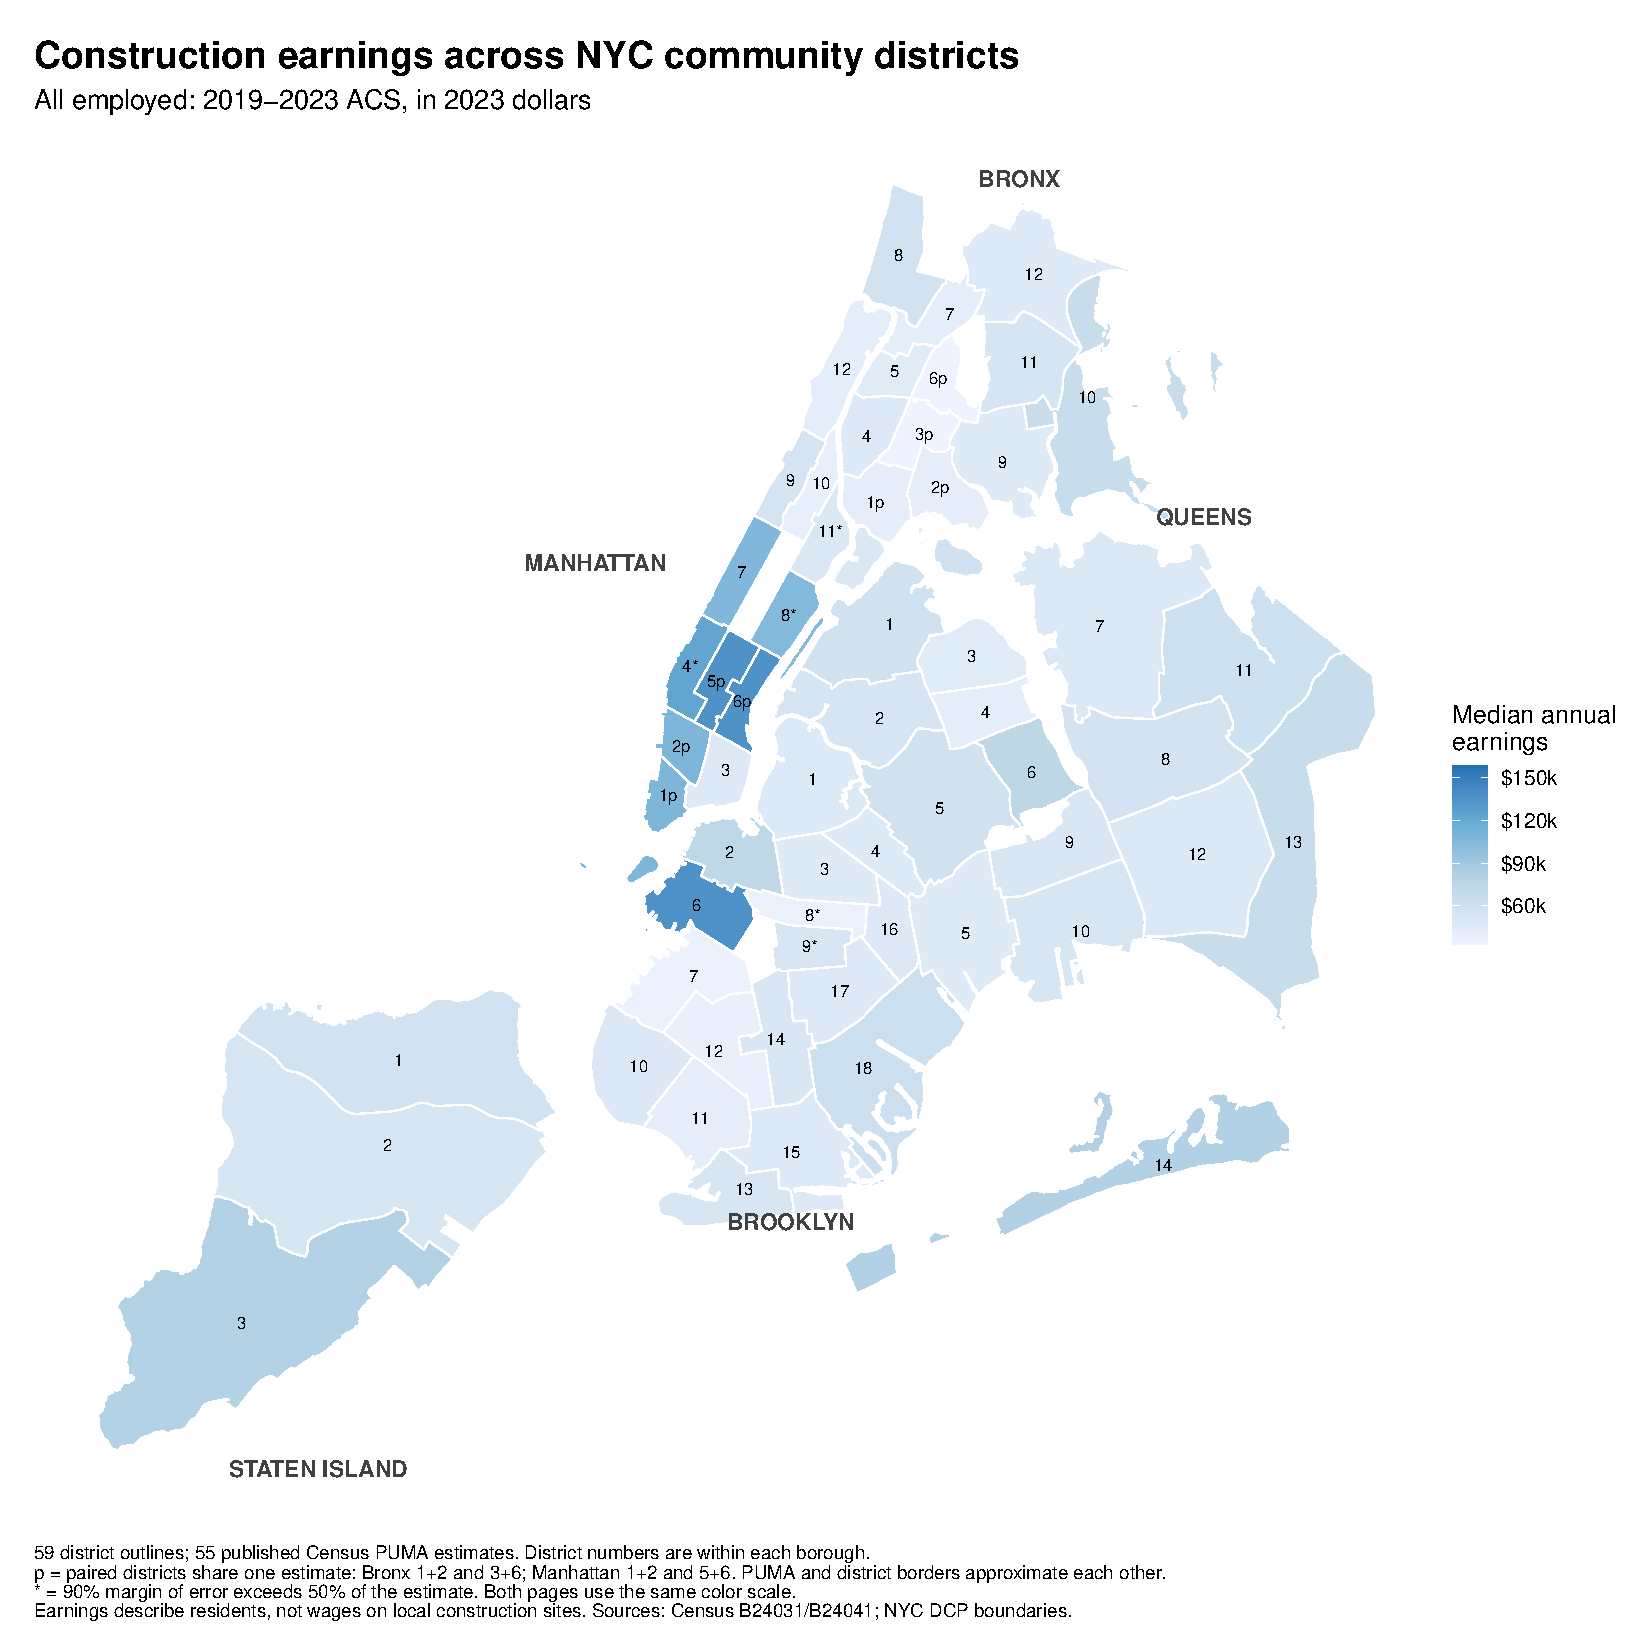
\includegraphics[page=1,width=\textwidth,height=.95\textheight,keepaspectratio]{archive/2026-09-08-wage-feasibility/community_district_earnings_map.pdf}
\end{center}
